\def\numbertoname#1{#1}
\def\remembernamevalue#1#2{}
\newcount\countRepos
\newcount\countMissingCode
\newcount\countCommentedOut
\newcount\countNotCommentedOut
\documentclass[11pt]{article}
\usepackage{geometry} 
\geometry{a4paper}  
\usepackage{graphicx}
\usepackage{amssymb}
\usepackage{epstopdf}
\usepackage{url}
\DeclareGraphicsRule{.tif}{png}{.png}{`convert \#1 `dirname #1`/`basename #1 .tif`.png}
\def\supplement{Supplement}
\begin{document}
\section{Section generated by \emph{Mathematica\/} taken from full paper}\subsection{The siren call of over-fitting code}\label{over-fit}
%Science is a methodical process that constructs principles and theories that describe the world, and competitive peer reviewed publication is the reliable record of that. We do the science, and we are in the world, so there are challenging meta-theoretical issues as well as practical experimental and resourcing issues. Karl Popper is one of many philosophers of science to develop principles and theories about science \cite{popper-three-worlds,popper-conjectures-refutations}. 

%Popper was concerned with the conventional sciences, where the world, Nature, is assumed fixed and in principle knowable. Writing just six years after Popper, Herbert Simon introduced the ``sciences of the artificial'' \cite{sciences-artificial}, which instead focus on understanding artificial worlds, most typically computer programs. Programs effectively create worlds, and the sciences of the artificial seek to understand and improve those worlds. Crucially, there is no philosophical or other reason why artificial worlds should be based on principles, let alone be simple or elegant. Conventional science's \ae sthetics need not apply.

%Science to date has been inevitably driven by human \ae sthetics: that is, simple, elegant, understandable, beautiful, brief, exciting, intelligible \ldots\ all are human properties that are applied to doing, funding, defining, and selecting ``good'' science. 

\noindent
Poor code undermines scientific quality: poor code can generate plausible results from \emph{any\/} data, including even fictional science. A temptation is that %artificial world \cite{sciences-artificial}, built on
adjusting the code's results gets more attention than the theoretical basis of the code's overall faithfulness to the experimental phenomena. \def\imageWidthCalculation{\multiply \imageWidth by 21 \divide \imageWidth by 28}
\def\figureStarDetails{*}
\begin{figure\figureStarDetails}[t]
{ \newdimen \imageWidth 
  \imageWidth=\textwidth
  \imageWidthCalculation
  \begin{center}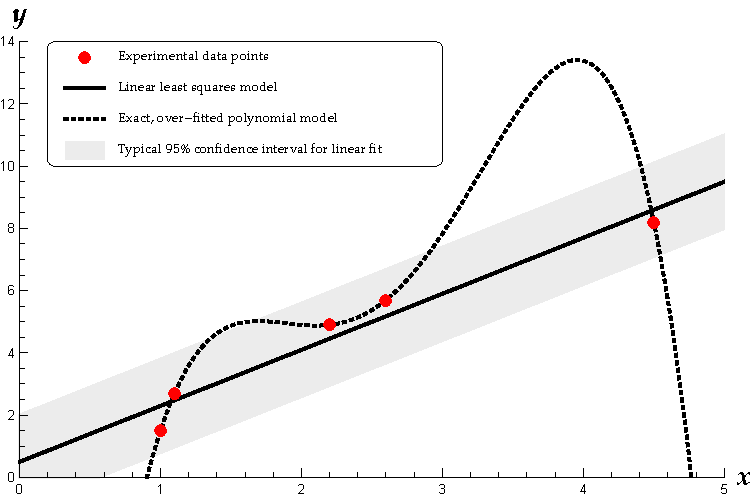
\includegraphics[width=\imageWidth]{generated/mathematicaplot.pdf}\end{center}}
\caption{Much computational science is concerned with finding plausible multi-dimensional models that fit models to data with the aim of extrapolating or predicting new results from them. Shown here is notional sample of experimental 2D data (the dots), a linear least squares regression, and an exact polynomial model. The over-fitted polynomial model fits the sample \emph{exactly\/}, but since the experimental data is presumably subject to random error (indicated by the confidence interval, itself estimated) the linear model would generally be considered a better description of the experimental data.}
\label{fig-overfit}
\end{figure\figureStarDetails}
In modeling terms, superficially successful computer programs tend to \emph{over-fit\/} phenomena \cite{over-fit}. Instead of using code to test the models, we tinker with the code adapting it closer and closer to our prejudices. The code then apparently confirms our science, since we fitted it to our understanding.  

In general, an \emph{over-fitted model\/} fits a set of data closely, but contains more parameters than can be justified by the science. An over-fitted model fails to reliably predict results beyond the scope of the data it has been fitted to. Over-fitting is a well-known problem, but the point is that when code is used, over-fitting is done unconsciously by programmers adjusting the code --- its parameters, its structure, its embedded data, the calculations it performs --- that specifies the model. ``A model over-fits if it is  more complex than another model that fits equally well'' \cite{over-fit}, is a criterion that describes almost every program! Programmers without the discipline and experience to manage the unlimited adaptability of code debug, alter, and extend their code to make it do what they think it should do. This becomes a vicious circle as the idea of what the science is becomes driven by the code. Rather than debugging code by improving its fit to the actual science, it gets debugged and extended to fit the expectations.  

The problems of over-fitting data may be visualized using a Real$\rightarrow$Real function of one variable (figure \ref{fig-overfit}). The code that generates an over-fitted curve seems to work very well: in the example shown, the over-fitted curve fits the sampled data exactly; indeed, the code used here will fit any new data exactly as well. But the code has a negligible ability to predict new data or to describe theories of the data, which is the point of modeling. The fact that over-fitted code seems to work well is deceptive.

Looking specifically at the data plotted in figure \ref{fig-overfit} if, for the sake of argument, we assume the error in the data is normally distributed then the values the over-fitted code generates outside the range of the sample are improbable. For example, the basic linear model predicts$\hat{y}(0)=0.5$, versus the extreme value predicted by the over-fitting code, $\hat{y}(0)=-41.8$,  even lies far outside the plot region shown in the figure.\footnote{The bounds of the confidence interval illustrated in figure \ref{fig-overfit} depend on assumptions about the distribution of the data; in this example, we are \emph{assuming}, perhaps because we know something more about the experiment, or thanks to Occam's Razor that a linear function is more likely than a high order polynomial.} Similar problems happen with interpolation rather than extrapolation, for instance around $x=4$.

While over-fitting data is a well-known problem, the point for this paper is that \emph{code\/} itself can easily be over-fitted. Code can of course be over-fitted in more complex ways than can be illustrated with elementary polynomials, as here. Code over-fitting is much harder to recognize because there may be no simple graph plot, like figure \ref{fig-overfit}, to highlight the problems. Furthermore, almost all code is far more intricate than the two trivial polynomials used to illustrated figure \ref{fig-overfit}. 

Unfortunately, code in published science \emph{is\/} often over-fitted, and over-fitted in a way that is very hard to scrutinize. For example, in epidemiology (which is considered in section \ref{section-pandemic-modeling}) it is routine to use very complicated, large dynamical models parameterized with numerous social, cultural, health, demographic and geographical data. The parameterization is mixed between data files, data written explicitly into the code, and with conditionals and other structuring in the code to cover special cases. Indeed, many of the programs in the survey used comment to inactivate code, presumably indicating an unfinished tinkering approach to code development.\footnote{Of the \the\countRepos\ papers in the pilot survey that reported use of code repositories (covering \input ../generated/kloc.tex
\totalkLOC\ thousand lines of code --- so this is not a trivial amount of programming effort), \numbertoname{\the\countMissingCode} provided an empty repository with no code at all (effectively commenting out all their code!), and \numbertoname{\the\countCommentedOut} repositories explicitly commented out chunks of workable code. The \numbertoname{\the\countNotCommentedOut} remaining non-trivial repositories with no commented-out code consisted of straightforward, short code files with few comments of any sort.\remembernamevalue{numbernamesexamplefootnote}{\thefootnote}}

Furthermore, scientific support code is rarely documented well enough to know what it should have been doing, which should be answered by a specification. With no clear specification and documentation, the code can be arbitrarily hacked to get any convenient results, since no particular specification for it has been defined that it should adhere to. Thus we risk doing and promoting substandard science because we --- the scientists and the publication process --- are not managing the unlimited adaptability and complexity of code that science has come to rely~on. This is over-fitting of the worst kind --- in conventional over-fitting one can at least hope to see that the fitting is over-parameterized for the data, but in code over-fitting the code and specification are not visible, therefore not adequately scrutinized, and --- worse --- the ``data'' the code over-fits includes the entire conceptual contribution of the paper. 

Reference \cite{may-simple} shows that even trivial code (in the case cited, implementing simple difference equations) with very few parameters can have very complex results, and reference \cite{dyson} is a historically significant example how pointing out the problem of over-fitting has improved science.
\vfill % the vfill is only needed to put the box at the bottom of a column if that makes it look better
\vskip 1ex
\noindent 
{\newdimen\boxwidth
\boxwidth = \columnwidth
\advance\boxwidth by - 1em
\begin{tabular}{@{}l@{}}
\framebox[\columnwidth][r]{\hfill\parbox{\boxwidth}{This section (\ref{over-fit}) of this paper, including figure \ref{fig-overfit}, was generated as a computational paper in a \emph{Mathematica\/} notebook, then exported to \LaTeX\ to include here. The \supplement\ provides a more complete explanation, as well as the data and details of the fitted polynomials (also generated automatically). This paper's repository includes the notebook.

%\hskip 1em Generated text and data presented elsewhere in this paper were created by a \texttt{make} file running shell scripts and JavaScript code analyzing repositories, JSON survey data, etc. Results were exported to files of \LaTeX\ markup and definitions, then imported into this paper and expanded where needed.
}\hfill}\end{tabular}}
\section{Data and polynomials}
\begin{center}\sf\begin{tabular}{|c|r|r|r|r|r|}\hline
$x={}$&1.00&1.10&2.20&2.60&4.50\\
$y={}$&1.50&2.70&4.90&5.70&8.20\\
\hline\end{tabular}
\end{center}

Showing both polynomials with coefficients to 2 decimal places, the linear least squares model to fit this data is:

$$
\hat{y}=0.49+1.80x
$$

and the Lagrange polynomial model (an exact fit to the 5 data points) is

$$
\hat{y}=-41.79+85.46x-56.30x^2+15.65x^3-1.51x^4
$$

The name of the relevant \emph{Mathematica\/} notebook file where all data and code for this section (and for generating the paper's section \ref{over-fit} and its figure \ref{fig-overfit}) can be found in \texttt{programs/over-fitting-section.nb}, which is included in the Git repository for the paper.\end{document}
